\RequirePackage{luatex85}
\documentclass[border={20pt,20pt,20pt,20pt}]{standalone}

\usepackage[dvipsnames]{xcolor}
\usepackage{tikz}
\usetikzlibrary{shapes, patterns, calc}

\begin{document}
	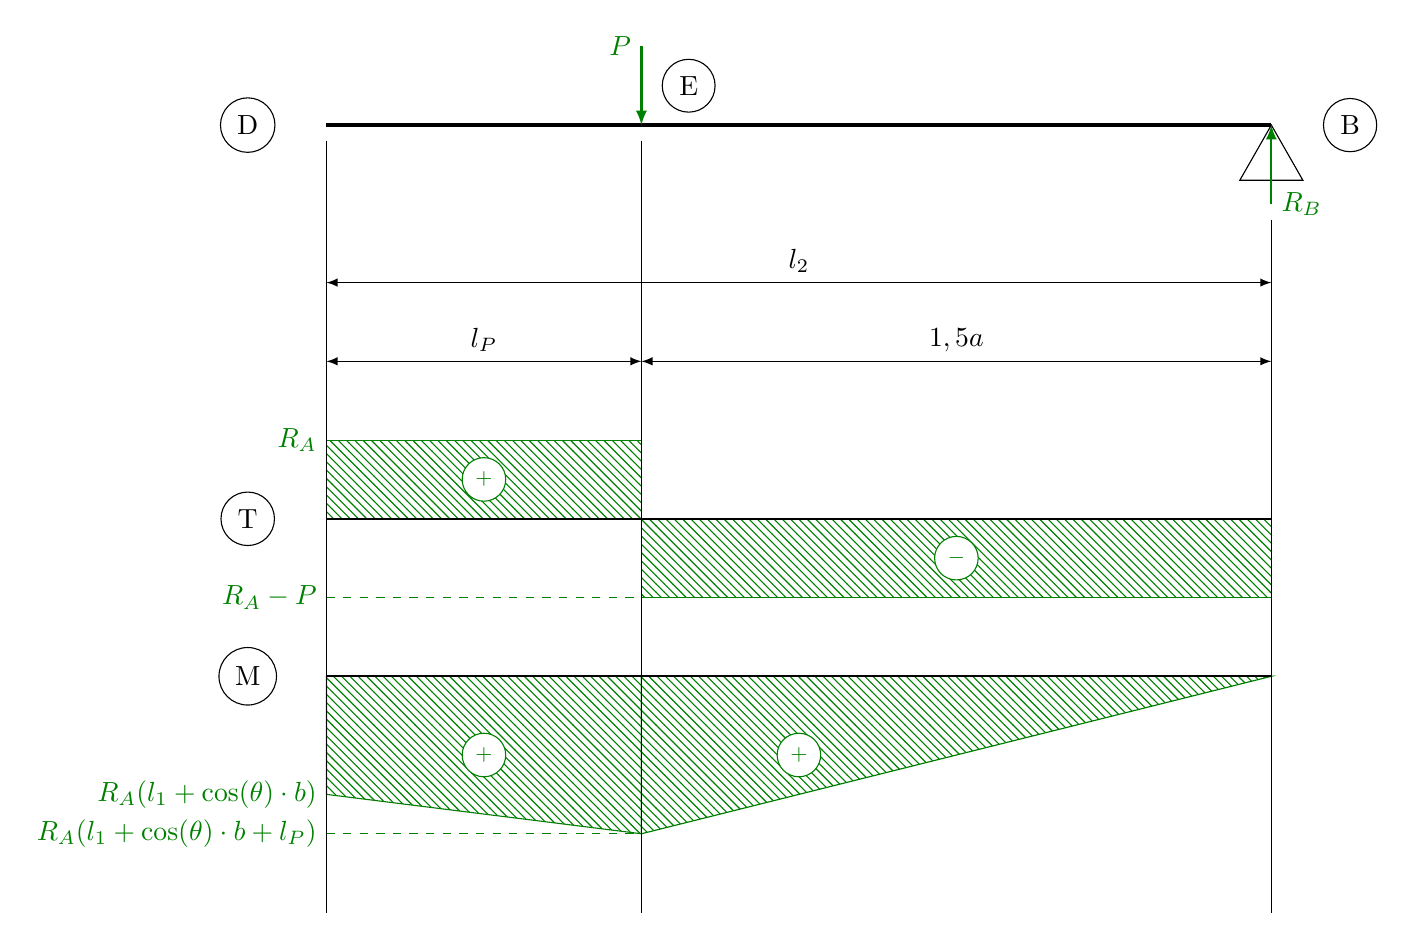
\begin{tikzpicture}[
	label/.style={circle,draw},
	gFill/.style={Green, pattern=north west lines, pattern color=Green},
	arrow/.style={latex-latex},
	inSymb/.style={Green, fill=white, circle, draw}
	]
	
	\coordinate (D) at (0, 0);
	\coordinate (E) at (4, 0);
	\coordinate (B) at (12, 0);
	
	\draw[very thick] (D) -- (B);
	\node [label] at ($(D) + (-1,0)$) {D};
	\node [label] at ($(E) + (.6, .5)$) {E};
	\node [label] at ($(B) + (1, 0)$) {B};
	
	\draw [arrow] ($(D) - (0, 2)$) -- ($(B) - (0, 2)$) node[midway, above] {$l_2$};
	\draw [arrow] ($(D) - (0, 3)$) -- ($(E) - (0, 3)$) node[midway, above] {$l_P$};
	\draw [arrow] ($(E) - (0, 3)$) -- ($(B) - (0, 3)$) node[midway, above] {$1,5a$};
	
	\draw (B) -- ($(B) - (.4,.7)$) -- ($(B) + (+.4, -.7)$) -- cycle;
	
	\coordinate (T1) at ($(D) - (0, 5)$);
	\coordinate (T2) at ($(E) - (0, 5)$);
	\coordinate (T21) at ($(T2) + (0, 1)$);
	\coordinate (T22) at ($(T2) - (0, 1)$);
	\coordinate (T3) at ($(B) - (0, 5)$);
	\coordinate (M1) at ($(T1) - (0, 2)$);
	\coordinate (M2) at ($(T2) - (0, 2)$);
	\coordinate (M21) at ($(M2) - (0, 2)$);
	\coordinate (M3) at ($(T3) - (0, 2)$);
	
	% Tallant
	\node [label] at ($(T1) - (1, 0)$) {T};
	\draw[gFill] (T1) rectangle ($(T2) + (0, 1)$);
	\draw[gFill] (T2) rectangle ($(T3) - (0, 1)$);
	\draw[thick] (T1) -- (T3);
	\node[Green, anchor=east] at ($(T1) + (0, 1)$) {$R_A$};
	\draw[Green, dashed] ($(T1) - (0, 1)$) -- ($(T2) - (0, 1)$);
	\node[Green, anchor=east] at ($(T1) - (0, 1)$) {$R_A - P$};
	\node[inSymb, scale=.8] at ($(T1)!.5!(T21)$) {$+$};
	\node[inSymb, scale=.8] at ($(T22)!.5!(T3)$) {$-$};
	
	
	% Moment
	\node [label] at ($(M1) - (1, 0)$) {M};
	\draw[gFill] (M1) -- ($(M1) - (0, 1.5)$) -- ($(M2) - (0, 2)$) -- (M2) -- cycle;
	\draw[gFill] (M2) -- ($(M2) - (0, 2)$) -- (M3) -- cycle;
	\draw[thick] (M1) -- (M3);
	\node[Green, anchor=east] at ($(M1) - (0, 1.5)$) {$R_A (l_1 + \cos(\theta) \cdot b)$};
	\draw[Green, dashed] ($(M1) - (0, 2)$) -- ($(M2) - (0, 2)$);
	\node[Green, anchor=east] at ($(M1) - (0, 2)$) {$R_A (l_1 + \cos(\theta) \cdot b + l_P)$};
	\node[inSymb, scale=.8] at ($(M1)!.5!(M21)$) {$+$};
	\node[inSymb, scale=.8] at ($(M21)!.5!(M3) - (2, 0)$) {$+$};
	
	\draw ($(D) - (0, .2)$) -- ($(M1) - (0, 3)$);
	\draw ($(E) - (0, .2)$) -- ($(M2) - (0, 3)$);
	\draw ($(B) - (0, 1.2)$) -- ($(M3) - (0, 3)$);
	
	\draw[Green, -latex, thick] ($(B) - (0, 1)$) -- (B) node[at start, right] {$R_B$};
	\draw[Green, -latex, thick] ($(E) + (0, 1)$) -- (E) node[at start, left] {$P$};
	\end{tikzpicture}
\end{document}